\documentclass{article}

\usepackage[utf8]{inputenc}
\usepackage[T1]{fontenc}

% Idioma
\usepackage[spanish,es-tabla]{babel}

% Matemática
\usepackage{amsmath, amssymb, mathtools}

% Gráficos
\usepackage{graphicx}
\usepackage{subcaption}

% Colores (cargar una sola vez)
\usepackage[table,xcdraw]{xcolor}

% Geometría
\usepackage[a4paper,margin=1in]{geometry}

% Links
\usepackage[hidelinks]{hyperref}

% Bibliografía
\usepackage[backend=bibtex]{biblatex}
\usepackage{csquotes}

% Símbolos
\usepackage{gensymb}

% =========================
% CONFIGURACIÓN VERILOG
% =========================
\usepackage{listings}

% Definición personalizada de Verilog/SystemVerilog
\lstdefinelanguage{Verilog}{
    morekeywords={
        module,endmodule,input,output,inout,wire,reg,logic,
        assign,always,always_ff,always_comb,if,else,case,endcase,
        begin,end,for,while,parameter,localparam
    },
    sensitive=true,
    morecomment=[l]{//},
    morecomment=[s]{/*}{*/},
    morestring=[b]"
}

\lstset{
    language=Verilog,
    basicstyle=\ttfamily\small,
    frame=single,
    numbers=left,
    numberstyle=\tiny,
    keywordstyle=\color{blue}\bfseries,
    commentstyle=\color{gray}\itshape,
    stringstyle=\color{green!50!black},
    breaklines=true,
    showstringspaces=false,
    tabsize=2,
    backgroundcolor=\color{gray!5}
}

% =========================

\addbibresource{bibliografia.bib} %archivo de bibliografia

\begin{document}

\renewcommand{\figureautorefname}{Fig.}
\renewcommand{\tableautorefname}{Tab.}
\renewcommand{\equationautorefname}{Ec.}

\begin{titlepage}

\thispagestyle{empty}

% Portada Custom, ver /maketitle: https://www.overleaf.com/learn/latex/How_to_Write_a_Thesis_in_LaTeX_(Part_5)%3A_Customising_Your_Title_Page_and_Abstract

\begin{center}
    
\includegraphics[width=5cm]{figures/unc_logo.png} \hspace{2cm}
    
\includegraphics[width=5.8cm]{figures/fcefyn_logo.jpg}
    \\[1cm]
    \vspace{5pt}
    \LARGE Fundación Fulgor\\[0.5cm] 
    \large Diseño Digital Avanzado \\[0.5cm] 
    \large GP01
    \\[0.2cm]
    %\large Trabajo Práctico N° 1
    \vspace{60pt}
    \begin{table}[!h]
    \centering
    \begin{tabular}{ll}
    \multicolumn{1}{c}{Nombre} & \multicolumn{1}{c}{DNI} \\
    Corvalán, Abel Nicolás & 41.220.050
    \end{tabular}
    \end{table}
    \vspace{20pt}
    \begin{table}[!h]
    \centering
    \begin{tabular}{ll}
    \multicolumn{1}{c}{Docentes} & Ing. Pola, Ariel \\
     & Cayuela, Pablo.
    \end{tabular}
    \end{table}
    \vfill
    Córdoba, República Argentina\\
    \today
\end{center}

\end{titlepage}
\newpage

\tableofcontents
\newpage
\listoffigures
\newpage
\listoftables

\newpage

\section{}

\section{Ejercicio 1}
% \begin{figure}[h!]
%     \centering
%     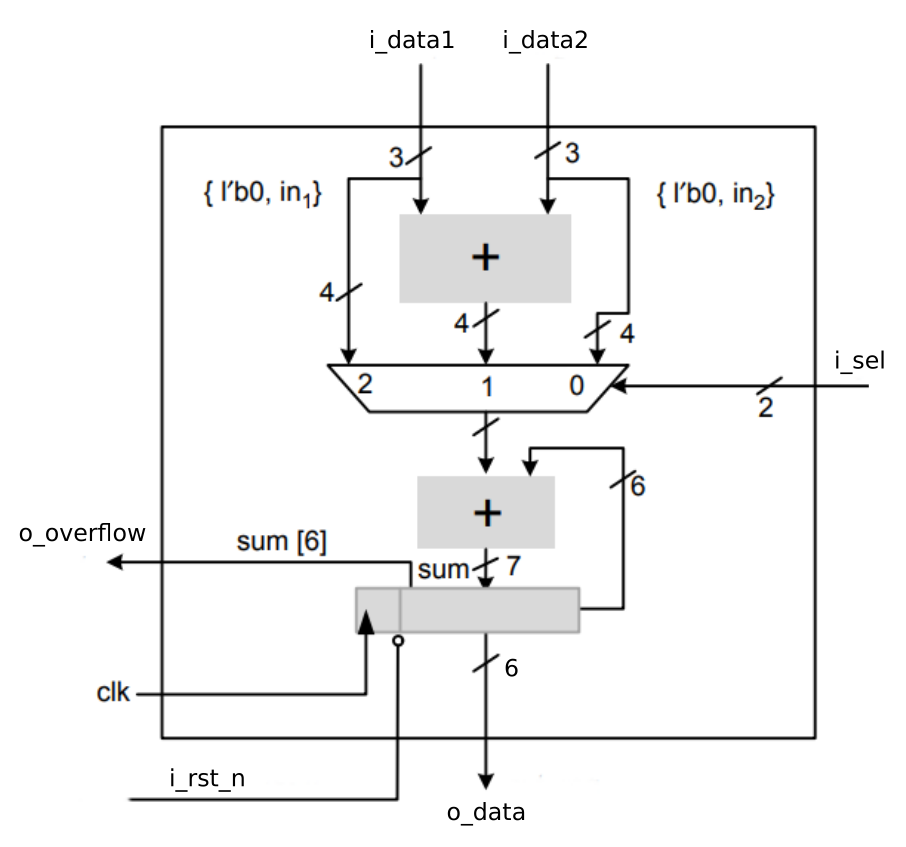
\includegraphics[width=0.5\linewidth]{img/esquemático1.png}
%     \caption{Esquemático del sistema}
%     \label{fig:esquematico1}
% \end{figure}

\subsection{Análsis de etapas}

\subsection{Consignas}

\begin{enumerate}
    \item Escribir el código Verilog para implementar el diseño de la Figura 1 considerando reset asíncrono.

Se modela el sistema en 4 módulos diferentes:

\begin{itemize}
    \item adder\_4b.
    \item adder\_7b.
    \item multiplexer.
    \item register1.
\end{itemize}

A continuación se muestra el código verilog de cada etapa:

\subsubsection{adder\_4b}

\begin{lstlisting}
module adder_4b(
    // Outputs.
    output wire [3:0]  o_sum1,
    // Inputs.
    input  wire [2:0] i_data1,
    input  wire [2:0] i_data2  
);

assign o_sum1 = i_data1 + i_data2;

endmodule    
\end{lstlisting}

\subsubsection{adder\_7b}

\begin{lstlisting}
module adder_7b(
    // Output.
    output [6:0] o_sum2,
    // Inputs.
    input  [5:0] i_sumA,
    input  [5:0] i_sumB
);
assign o_sum2 = i_sumA + i_sumB;
endmodule
\end{lstlisting}

\subsubsection{multiplexer}

\begin{lstlisting}
module multiplexer(
    // Outputs.
    output reg  [3:0] o_multiplexer,
    // Inputs.
    input       [3:0] i_0          ,
    input       [3:0] i_1          ,
    input       [3:0] i_2          ,
    input       [1:0] i_sel        
);

always@(*) begin
    case (i_sel)
        2'b00:   o_multiplexer = i_0;
        2'b01:   o_multiplexer = i_1; 
        2'b10:   o_multiplexer = i_2;
        default: o_multiplexer = 4'b0000;
    endcase
end
endmodule
\end{lstlisting}

\subsubsection{register1}

\begin{lstlisting}
module register1(

    // Output.
    output reg [5:0] o_data    , // Output
    output reg       o_overflow, // Overflow
    // Inputs.
    input      [6:0] i_sum     , // Input
    input            clk       , // Clock Signal
    input            i_rst_n     // Negative Reset Signal
);

    always @(posedge clk or i_rst_n) begin
        if(!i_rst_n) begin
            o_data     = 6'b000000 ;
            o_overflow = 1'b0      ; 
        end else begin 
            //o_data     <= i_sum[5:0];
            //o_overflow <= i_sum[6]  ;
            {o_overflow, o_data} = i_sum;
        end
    end
endmodule
\end{lstlisting}

\subsubsection{top}

\begin{lstlisting}
module top(
    // Outputs.
    output [5:0] o_data    ,
    output       o_overflow,
    // Inputs.
    input  [2:0] i_data1   ,
    input  [2:0] i_data2   ,
    input  [1:0] i_sel     ,
    input        clk       ,
    input        i_rst_n
);

adder_4b
    adder_4b(
        .o_sum1  (o_sum1) ,

        .i_data1 (i_data1),
        .i_data2 (i_data2)
    );
    
wire [3:0] i_0;
wire [3:0] o_sum1;
wire [3:0] i_2;

assign i_0 = {1'b0, i_data2};
assign i_2 = {1'b0, i_data1};

multiplexer
    multiplexer(
        .o_multiplexer(o_multiplexer),
        
        .i_0          (i_0)   ,
        .i_1          (o_sum1),
        .i_2          (i_2)   ,
        .i_sel        (i_sel)
    );

wire [3:0] o_multiplexer;
wire [5:0] i_sum2 = {2'b00, o_multiplexer};

adder_7b
    adder_7b(
        .o_sum2       (o_sum2)       ,
        .i_sumA       (i_sum2)       ,
        .i_sumB       (o_data) // connect with output of register1.
    );

wire [6:0] o_sum2;

register1
    register1(
        .o_data       (o_data)    ,
        .o_overflow   (o_overflow),
   
        .i_sum        (o_sum2)    ,
        .clk          (clk)       ,
        .i_rst_n      (i_rst_n)
    );
endmodule
\end{lstlisting}
    
    \item Genere la señal de reset apropiada para el registro de realimentación utilizado en el diseño.

En el módulo $register1.v$ se diseña el reset asíncrono del sistema. A continuación se muestra el código verilog con el bloque procedural que contiene la señal de reset $i\_rst\_n$.

\begin{lstlisting}
always @(posedge clk or i_rst_n) begin
    if(!i_rst_n) begin
        o_data     = 6'b000000 ;
        o_overflow = 1'b0      ; 
    end else begin 
        //o_data     <= i_sum[5:0];
        //o_overflow <= i_sum[6]  ;
        {o_overflow, o_data} = i_sum;
    end
end    
\end{lstlisting}
    
    \item Escribir un testbench que permita verificar el correcto funcionamiento del circuito propuesto. Los estímulos pueden ser generados con python o modelados en el testbench.

Se genera el siguiente código test bench para verificar el correcto funcionamiento del sistema propuesto:

\begin{lstlisting}
`timescale 1ns/1ps

module tb_top();

wire [5:0] o_data    ;
wire       o_overflow;

reg  [2:0] i_data1   ;
reg  [2:0] i_data2   ;

reg  [1:0] i_sel     ;
reg        clk       ;
reg        i_rst_n   ;

top
    top(
        .o_data     (o_data)    ,
        .o_overflow (o_overflow),
        .i_data1    (i_data1)   ,
        .i_data2    (i_data2)   ,
        .i_sel      (i_sel)     ,   
        .clk        (clk)       ,
        .i_rst_n    (i_rst_n)
    );

initial begin
    clk     = 1'b0;
    i_data1 = 3'b000;
    i_data2 = 3'b000;
    i_sel   = 2'd0;
    i_rst_n = 1'b1;
end

always begin
    #5 clk = ~clk;
end

initial begin
    #10 i_data1 = 3'd2; i_data2 = 3'd2; 
    #10 i_data1 = 3'd1; i_data2 = 3'd1;
    #2 i_rst_n  = 1'b0;
    #10 i_data1 = 3'd5; i_data2 = 3'd5;
    #10 i_data1 = 3'd5; i_data2 = 3'd5;
    #4  i_rst_n = 1'b1;
    #10 i_sel   = 2'd1;
    #5  i_data1 = 3'd1; i_data2 = 3'd1;   
    #30;
    $finish;
end
endmodule
\end{lstlisting}

    \item ¿Cuantos ciclos de reloj son necesarios para que el registro $o\_data$ produzca overflow cuando $i\_sel$, $i\_data1$ e $i\_data2$ son iguales a 1?
\newline
\newline
Para obtener la cantidad de ciclos necesarios para que el registro produzca overflow se escribe el siguiente código test bench de descripción de hardware en lenguaje Verilog.
\newline

% Código de test bench.
\begin{lstlisting}
`timescale 1ns/1ps

module tb_top();
wire [5:0] o_data    ;
wire       o_overflow;

reg  [2:0] i_data1   ;
reg  [2:0] i_data2   ;

reg  [1:0] i_sel     ;
reg        clk       ;
reg        i_rst_n   ;

top
    top(
        .o_data     (o_data)    ,
        .o_overflow (o_overflow),
        .i_data1    (i_data1)   ,
        .i_data2    (i_data2)   ,
        .i_sel      (i_sel)     ,   
        .clk        (clk)       ,
        .i_rst_n    (i_rst_n)
    );

initial begin
    clk     = 1'b0;
    i_data1 = 3'b000;
    i_data2 = 3'b000;
    i_sel   = 2'd0;
    i_rst_n = 1'b1;
end

always begin
    #5 clk = ~clk;
end

initial begin
    #10 i_data1 = 3'd2; i_data2 = 3'd2; 
    #10 i_data1 = 3'd1; i_data2 = 3'd1;
    #2 i_rst_n  = 1'b0;

    #10 i_data1 = 3'd5; i_data2 = 3'd5;
    #10 i_data1 = 3'd5; i_data2 = 3'd5;

    #4  i_rst_n = 1'b1;
    #10 i_sel   = 2'd1;
    #5  i_data1 = 3'd1; i_data2 = 3'd1;  
    #30;
    $finish;
end
endmodule
\end{lstlisting}

Se obtiene el siguiente diagrama de onda para el test bench con las señales pedidas:

% \begin{figure}[h!]
%     \centering
%     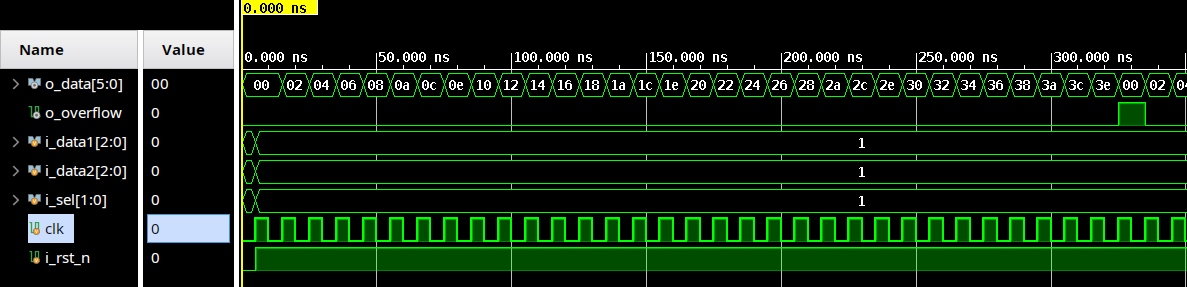
\includegraphics[width=1.0\linewidth]{img/ejercicio1_punto4.png}   \caption{Diagrama de onda, overflow en sistema}
%     \label{fig:onda-overflow}
% \end{figure}

Se tiene que un periodo de la señal de clock $clk$ es igual a $10 \, seg$. Hay 32 ciclos hasta que se produzca el overflow con las condiciones $i\_sel=1$, $i\_data1= 1$, $i\_data2= 1$.

$$ Ciclos_{overflow}\frac{t_{overflow}}{T_{ciclo}}=\frac{320ns}{10ns}= 32 \, ciclos$$

$$ \boxed{ Ciclos_{overflow}= 32 \, ciclos }$$

\end{enumerate}

\section{Ejercicio 2}

\begin{enumerate}
    \item Realizar el esquemático o diagrama en bloque del datapath de un selector de operaciones que ejecuta las siguientes operaciones aritméticas en paralelo con dos entradas $i\_dataA$ e $i\_dataB$ de tipo signadas de $16 bits$ y asigne el valor del resultado a una salida $o\_dataC$ de $16 \, bits$.

    \item La elección de la operación a realizar depende de una señal de control $i\_sel$ de $2 \, bits$.

    \item Implementar el diseño en Verilog y el testbench para verificar el comportamiento.

    Operaciones:

        $$o\_dataC \, = i\_dataA \, + \, i\_dataB $$
        $$o\_dataC \, = i\_dataA \, - \, i\_dataB $$
        $$o\_dataC \, = i\_dataA \, \& \, i\_dataB $$
        $$o\_dataC \, = i\_dataA \, | \, i\_dataB $$


% \begin{figure}[h!]
%     \centering
%     
\includegraphics[width=1.0\linewidth]{{img/Diagrama de onda, sistema de operaciones}.png}
%     \caption{Diagrama de onda, sistema de operaciones}
%     \label{fig:onda-operaciones}
% \end{figure}

% \begin{figure}[h!]
%     \centering
%     
\includegraphics[width=1.0\linewidth]{{img/Diagrama de ondas, sistema en hexadecimal}.png}
%     \caption{Diagrama de onda, sistema de operaciones hexadecimal}
%     \label{fig:onda-operaciones-hex}
% \end{figure}
    
\end{enumerate}
\section{Ejercicio 3}

Dibuje el esquemático para el siguiente código Verilog. Especifique de forma clara los tamaños de datos para todos los cables y muestre multiplexores, registros, señales de clock y reset.

\begin{lstlisting}
module test_module(
    input      [31:0]   x0,
    input      [1:0]    sel,
    input               clk,
    input               rst_n,
    output reg [31:0]   y0
);

reg  [31:0] x1, x2, x3;
reg  [31:0] y1;
wire [31:0] out;

assign out = (x0 + x1 + x2 + x3 + y1) >>> 2;

always @(posedge clk or negedge rst_n) begin
    if (!rst_n) begin
        x1 <= 0;
        x2 <= 0;
        x3 <= 0;
    end
    else if (sel == 0) begin
        x3 <= x2;
        x2 <= x1;
        x1 <= x0;
    end
    else if (sel == 01) begin
        x3 <= x1;
        x2 <= x0;
        x1 <= x2;
    end
    else begin
        x3 <= x3;
        x2 <= x2;
        x1 <= x0;
    end
end

always @(posedge clk or negedge rst_n) begin
    if (!rst_n) begin
        y1 <= 0;
        y0 <= 0;
    end
    else begin
        y1 <= y0;
        y0 <= out;
    end
end
endmodule
\end{lstlisting}

Este codigo modela y describe un filtro promedio (moving average) con realimentacion. Es un sistema IIR (Infinite Impulse Response) a causa de la realimentacion $y[n-1]$. No depende solo de las entradas pasadas.


\section{Ejercicio 4}

$$ y[n]= x[n] - x[n-1] + x[n-2] + x[n-3] + 0.5 y[n-1] + 0.25 y[n-2] $$

\begin{itemize}
    \item Dibujar la arquitectura de la siguiente ecuación diferencial.

% Pasar esquema.

    \item Escribir el código Verilog.

Código de descripción del filtro IIR con entrada de 8 bits (incluyendo signo).

\begin{lstlisting}[]
module top(
    // Output
    output reg signed [10:0] y ,
    // Delayed inputs
    output reg signed [7:0]  x1,
    output reg signed [7:0]  x2,
    output reg signed [7:0]  x3,
    // Outputs for debug
    output reg signed [10:0] y1,
    output reg signed [10:0] y2,
    // Input
    input signed [7:0] x,
    input clk, 
    input rst_n
);

// We need 11 bits to representate 
// -512 to 512
wire signed [10:0] y_o;

// Equation implementation
assign y_o = x - x1 + x2 + x3 + (y1 >>> 1) + (y2 >>> 2);

always @(posedge clk or negedge rst_n) begin
    if(!rst_n) begin
        x1 <= 0;
        x2 <= 0;
        x3 <= 0;
        y  <= 0;
        y1 <= 0;
        y2 <= 0;
    end else begin
        // Shift registers for input
        x1 <= x;
        x2 <= x1;
        x3 <= x2;

        // Output
        y <= y_o;

        // Feedback paths
        y1 <= y_o;
        y2 <= y1;
    end
end

endmodule
\end{lstlisting}
\newpage
Código de testbench para el sistema.

\begin{lstlisting}
`timescale 1ns/1ps

module tb_top();

wire signed [10:0] out;

wire signed [7:0]  x1;
wire signed [7:0]  x2;
wire signed [7:0]  x3;

wire signed [10:0] y1;
wire signed [10:0] y2;

reg  signed [7:0]  x;
reg                clk;
reg                rst_n;

always #5 clk = ~clk;

initial begin
    clk   = 0;
    rst_n = 0;
    x    = -8'sd128;

    #20 rst_n = 1;

    // Repeat this block 256 times.
    // Control event on x.
    // This block increment the value of x.
    repeat(256) begin
        @(posedge clk);
        x = x + 1;
    end
    #100 $stop;
end
top
    top(
        .y(out),
        .x1(x1),
        .x2(x2),
        .x3(x3),
        .y1(y1),   
        .y2(y2),   
        .x(x),
        .clk(clk),
        .rst_n(rst_n)
    );
endmodule
\end{lstlisting}

A continuación se muestra el diagrama de onda del filtro IIR

% \begin{figure}[h!]
%     \centering
%     
\includegraphics[width=1.0\linewidth]{{img/Diagrama de onda, filtro IIR}.png}
%     \caption{Diagrama de onda, filtro IIR}
%     \label{fig:onda-iir}
% \end{figure}

    \item Considerar valores enteros en las muestras de entrada.

    \item Considerar 8bits para la representación de x y calcular el número de bits para la salida considerando full-resolution.

Se consideran 8 bits con signo para la entrada $x[n]$ en la salida se debería tener 11 bits, esto se debe a que:
 
El valor máximo y mínimo que se puede tener en la entrada por los siguientes cálculos:

$$ \boxed{ X_{max}= 2^{b-1}-1 } $$ \space \space \space \space $$ \boxed{ X_{min}= -2^{b-1} } $$

Siendo $b= 8 \, bits $.

$$ X_{max}= 2^{8-1}-1 = 127 $$
$$ \boxed{ X_{max}=127 } $$
$$ X_{min}= -2^{b-1} = -128 $$
$$ \boxed{ X_{min}= -128} $$

Se realiza el análisis de crecimiento de bits de la salida respecto de los valores de entrada.

\subsubsection{Camino directo (términos de entrada)}

Se considera el valor máximo positivo para la suma de términos. Esto es:

\begin{center}
\begin{tabular}{|c|c|c|c|}
    \hline
    x[n]      & x[n-1] & x[n-2] & x[n-3] \\ \hline
    $X_{max}$ & $X_{min}$ & $X_{max}$ & $X_{max}$ \\  \hline
\end{tabular}
\end{center}

Entonces el valor máximo positivo para la suma de términos de entrada será $23$.

$$ Max \, value \, of \, addition= 4X_{max} = 4(2^{b-1}-1) = 4(2^{8-1}-1) = 508   $$

Por lo que, en primer instancia, se necesitan 10 bits.

Se consideran los valores mínimos para la entrada.

\begin{center}
\begin{tabular}{|c|c|c|c|}
    \hline
    x[n]      & x[n-1] & x[n-2] & x[n-3] \\ \hline
    $X_{min}$ & $X_{max}$ & $X_{min}$ & $X_{min}$ \\  \hline
\end{tabular}
\end{center}

Entonces la magnitud de la suma máxima negativa será:

$$ Min \, value \, of \, addition= 4X_{min} = 4(2^{b-1}) = -4(2^{8-1}) = -512 $$

Se necesitan 10 bits para representar el valor mínimo.

La cantidad de bits necesaria para representar el rango de números de $-512$ a $508$ es:

$$ \boxed{ n= 10 \, bits } $$ %11 bits

\subsubsection{Camino de realimentación}

En el camino de realimentación se tienen las siguientes operaciones:

$$ 0.5y[n-1]+0.25y[n-2] $$

%Se establece que se requieren menos de $m \, bits$ para la representación de valores ya que los valores de $y$ con sus respectivos delay son multiplicados por coeficientes menores a 1 $(coef<1)$.

Se debe tener en cuenta que los valores de $y$ con sus respectivos delay son multiplicados por coeficientes menores a 1 $(coef<1)$. Lo cual reduce el valor y por lo tanto se reduce la cantidad de bits.

Para máxima resolución se considera el peor caso. Esto último sucede cuando la salida anterior se encuentra en su valor máximo. Si la salida es $Y_{max}$ entonces se tiene:

$$ 0.5Y_{max}+0.25Y_{max} = 0.75 \, Y_{max} $$

\subsubsection{Cálculo del peor caso total}

Se plantea el valor máximo absoluto:

$$ Y_{max}= 512 + 0.75Y_{max} $$

$$ Y_{max}(1-0.75) = 512 $$

$$ 0.25Y_{max}= 512 $$

$$ Y_{max}= 2048 $$

Entonces la cantidad necesaria de bits para representar la salida son los siguientes:

$$ 2048= 2^{11} $$

$$ \boxed{ cantidad \, de \, bits = 12 bits } $$

Se necesitan 12 bits para representar -2048.

Rango de salida de $[-2048, +2047]$.

Se obtienen los siguientes resultados:

\begin{center}
\begin{tabular}{|c|c|c|c|}
   \hline
   \multicolumn{2}{|c|}{Entrada} & \multicolumn{2}{|c|}{Salida}  \\ 
   \hline
   Valor mínimo & Valor máximo & Valor mínimo & Valor máximo \\ 
   \hline
   -128 & -127 & -2048 & +2047 \\ 
   \hline
\end{tabular}
\end{center}

\end{itemize}

\section{LABORATORIO 2 - FEC - Grupo 1}

\subsection{Ejercicio 1 - Matrices y parámetros}

Escribir $\textbf{G}$ y $\textbf{H}$ a partir de $\textbf{B}$ y verificar que $\textbf{GH}^{T}= 0$ y $B^{2}=1$. Indicar dimensión, tasa y \textbf{overhead}. Codificar a mano $m=0xA5C$ y comprobar que la palabra obtenida cumple $\textbf{vH}^{T}=0$.

\subsection{Ejercicio 2 - Distancia mínima y capacidad de corrección}

Determinar la distancia mínima, la capacidad de corrección $t$ y la capacidad de detección a partir de la distribución de pesos del código:


La distancia mínima es:

$$ d_{min}= 8 $$

La capacidad de corrección del código es:

$$ \boxed{t = \frac{d_{min}-1}{2}} $$

$$ t = \frac{8-1}{2}= \frac{7}{2}=3.5 \approx 3 $$

$$ \boxed{t= 3} $$

La capacidad de detección:

$$ capac. \, \, deteccion  = d_{min} - 1  $$

$$ capac. \, \, deteccion  = 8 - 1 = 7 $$

$$ \boxed{ capac. \, \, deteccion = 7 } $$

La capacidad de detección está determinada por la distancia mínima menos uno debido a que si nuestra codeword se modificó en, por ejemplo 7 bits, entonces se tiene que el resultado no pertenece a una codeword.



\printbibliography
\end{document}